% !TeX root = ../../../main.tex
\subsection{More Details on Experiments}
\label{ch02:sec:experiment-details}

\ChTwoHeadingOnly
\subsubsection{Baselines}
\label{ch02:sec:baselines}
In this section we describe the baselines used for our experiments.
We divide these baselines into 3 subgroups of: (a) Purely-supervised, (b) Predictive clustering, and (c) Self-supervised learning and contrastive learning methods.

\begin{itemize}
    \item \textbf{Purely-Supervised Baselines}
    
\end{itemize}
% \vspace{.2em}
\noindent
\textbf{Logistic regression.}
For this simple baseline, our training data has each timestep as an individual datapoint with the true label of each timestep being the final timestep outcome of its corresponding sequence. 
We run logistic regression on raw features of every timestep in the training set.


\noindent
\textbf{Long short-term memory (LSTM).}
We train a multilayer LSTM \citep{hochreiter1997long} on the sequences of the raw features in the training set and their corresponding outcome label and take the hidden layer of the final timestep and pass it through a linear layer to predict the outcome of the corresponding sequence.
After the training is completed, we run our model on the validation set and get the probability of the positive outcome (not surviving) for each sequence.


\noindent
\textbf{Reverse Time Attention Model (RETAIN).}
\citet{choi2016retain} proposed an interpretable predictive model for healthcare using reverse time attention mechanism. Their proposed model is based on a two-level neural attention model. It detects influential past visits and significant clinical variables within those visits by mimicking physician practice. The model attends to the EHR data in a reverse time order, giving higher attention to recent clinical measurements.


\noindent
\textbf{Diagnosis prediction in healthcare via attention-based bidirectional recurrent neural networks (DIPOLE).}
\citet{ma2017dipole} propose a model that utilizes bidirectional recurrent neural networks to remember all the information of both the past visits and the future visits. The authors introduce three attention mechanisms to measure the relationships of different visits for the prediction. Dipole uses the attention mechanism to interpret the prediction results it generates.


{\raggedright
\noindent
\textbf{Transformer: Bidirectional Encoder Representations from Transformers (BERT).} 
We train a BERT-based \citep{devlin2018bert} model from scratch to encode the time-series data of our experiments to predict the final outcome of each time-series.\par
}


\begin{itemize}
    \item \textbf{Predictive-Clustering Baselines}
    
\end{itemize}
% \vspace{.2em}
\noindent
\textbf{Actor-Critic Temporal Predictive Clustering (AC-TPC).}
\citet{lee2020temporal} proposed an actor-critic approach from reinforcement learning for temporal predictive clustering (AC-TPC) where each cluster consists of patients with similar future outcomes of interest.
In this approach an RNN-based encoder and multi-layer perceptron predictor network are first trained to initialize time series embeddings.
After initialization, a selector network and an embedding dictionary are jointly optimized with the encoder and predictor networks to obtain a representative embedding for each timestep, considering the outcome in the subsequent timestep.
During inference at each timestep, the encoder maps a sequence into a latent embedding.
Subsequently, the selector network assigns a cluster to this latent embedding.
The centroid of the cluster assigned to the latent embedding is stored in the embedding dictionary and used by the predictor network to make predictions regarding the future outcome of interest.


\noindent
\textbf{T-Phenotype.}
\citet{qin2023t} proposed a method for temporal clustering designed to uncover predictive temporal patterns from labeled time-series data, aiding in understanding disease progression. This method focuses on processing multivariate time-series data to extract predictive patterns and associate them with relevant clinical progression markers. At the heart of T-Phenotype is the utilization of the Laplace transform for representation learning, which transforms variable-length, irregularly sampled time-series data into a consistent and unified embedding in the frequency domain. This transformation is crucial for handling the inherent variability and complexity of clinical data. The model further includes a path-based similarity score, a novel metric to assess the relationship between temporal patterns and specific disease statuses. This score is instrumental in determining the relevance and predictive power of identified patterns. T-Phenotype then employs a graph-constrained K-means clustering process, guided by the path-based similarity graph, to categorize patients into distinct phenotypes. These phenotypes are defined by their unique temporal patterns, providing insights into different trajectories of disease progression and offering potential for personalized patient care strategies.

\begin{itemize}
    \item \textbf{Self-Supervised Learning and Contrastive Learning Baselines}
    
\end{itemize}
% \vspace{.2em}
\noindent
\textbf{Sequential Multi-Dimensional Self-Supervised Learning (SMD-SSL).}
\citet{raghu2023sequential} developed Sequential Multi-Dimensional Self-Supervised Learning (SMD-SSL) to effectively process complex clinical time series data, particularly in settings with abundant multimodal data like intensive care units. This method addresses the shortcomings of traditional self-supervised learning approaches that are limited to unimodal data. SMD-SSL is capable of handling both structured data, such as lab values and vital signs, and high-dimensional physiological signals like electrocardiograms. It employs a dual SSL loss optimization strategy, applying one loss at the level of individual high-dimensional data points and another at the overall sequence level, enabling a more nuanced understanding of the multimodal clinical data. Crucially, SMD-SSL is designed to be compatible with different loss functions, allowing the use of either contrastive methods, as exemplified by SimCLR \citep{chen2020simple}, or non-contrastive approaches like VICReg \citep{bardes2021vicreg}. In our experiments, we implement SMD-SSL using both the contrastive loss from SimCLR and the non-contrastive loss from VICReg. Following the self-supervised learning phase with each of these loss functions, we attach a prediction head to the model for our prediction tasks. We present two variations of the model in our experiments: a fine-tuned version, where the loss is back-propagated through both the prediction head and the main SMD-SSL encoder, and a frozen version, in which we keep the main SMD-SSL encoder weights constant and optimize only the prediction head.


\noindent
\textbf{\ChTwoSmallCaps{Simple}-Supervised Contrastive Learning ({\ChTwoSmallCaps{Simple-SCL}})}
This baseline lies under the umbrella of embedding-centric models. \ChTwoSmallCaps{Simple-SCL} is a special case of the original \ChTwoSmallCaps{SCL} \citep{khosla2020supervised} which does not use data augmentation.
Similar to the original \ChTwoSmallCaps{SCL} it includes both an encoder network that first learns the embeddings and then a predictor network is trained on these learned embeddings to make predictions.
In our experiments that deals with temporal data, we treat each time step as an individual data point to train the encoder and predictor networks. \emph{Note that \ChTwoSmallCaps{Simple-SCL} can be viewed as an ablation of our full \ChTwoSmallCaps{Temporal-SCL} model that excludes both the temporal network and the nearest neighbor pairing mechanism.}  

\subsubsection{Experimental Setup Details}
\label{ch02:sec:ExperimentalSetup}

For all datasets, we randomly split the data into 60\% training, 20\% validation, and 20\% test sets. 
This split is done at the patient level.
The presented results of our experiments in the following sections would be for holdout test patients from which no training data was available.
We train our model on the patients in the training set, optimize the hyperparameters on the patients in the validation set and report the results from the holdout patient test set. 
We train each method on the training set, tune hyperparameters based on the validation set, and report evaluation metrics on the test set.
Furthermore, we choose 10 different random seeds to randomize the parameter initialization of all the models evaluated as well as randomizing the train/validation/test sets for each experimental repeat.

% \subsubsection{Evaluation Metrics}
% \label{sec:performance_metrics}

\noindent
\textbf{Evaluation metrics.}
We use the same evaluation metrics as \citet{lee2020temporal}.
To evaluate the supervised performance of our model and the baselines, we use area under receiver operator characteristic curve (AUROC) and area under precision-recall curve (AUPRC) obtained from the label predictions of our model and the ground-truth labels on the outcomes of interest. We use one-vs-rest AUROC and AUPRC.
For the synthetic data experiment, we also look at the fraction of experimental repeats that a method recovers the ground truth structure.
We also report the Silhouette index \citep{rousseeuw1987silhouettes} that gives us a measure of how similar a member is to its own cluster (homogeneity within a cluster) compared to other clusters (heterogeneity across clusters). 

In the ablation studies presented in Section~\ref{ch02:sec:ablation}, we also evaluate the unsupervised performance of different ablations of \ChTwoSmallCaps{Temporal-SCL}.
We cluster on the learned hyperspherical embeddings using a complete linkage Agglomerative Hierarchical Clustering to discover discrete latent states that could be of interest.  
We utilize three standard metrics for the scenario when ground-truth label is known and a fourth completely unsupervised metric.
The metrics used are purity score, normalized mutual information (NMI), adjusted rand index (ARI), and silhouette index (SI).
Purity score ranges from 0 to 1 and explains the homogeneity of each cluster with regards to the labels.
NMI ranges from 0 to 1 and is an information theoretic measure of mutual information shared between the labels and the cluster and is adjusted for the number of clusters with 1 being perfect clustering.
ARI ranges from -1 to 1 and evaluates the percentage of correct cluster assignments where 0 corresponds to completely random assignment and 1 being perfect clustering.
Lastly, SI is a completely unsupervised metric ranging from -1 to 1 which provides a simultaneous measure of (1) how similar members of a cluster are to their own cluster capturing the homogeneity within a cluster and (2) how different members of each cluster are compared to other clusters capturing heterogeneity across different clusters.


\noindent
\textbf{Training hyperparameters.}
% \label{sec:TrainingDetails}
Table~\ref{ch02:tab:trainingHyperParams} summarizes the hyperparameters used in all our experimentations presented in this paper.
{
% Please add the following required packages to your document preamble:
% \usepackage{multirow}

% !TeX root = ../../../main.tex
\begin{table}[!ht]
\caption{Training Details and Hyperparamters for Experiments.}
\centering
\begin{tabular}{|l|l|}
\hline
\textbf{Experiment}                    & \textbf{Synthetic Dataset}                                                                                                             \\ \hline
\textit{Main Network}                  & 2-Layer FCN ReLU Activation                                                                                                            \\
\textit{Main Network Layer Size}       & (input-dimension)2→16→3(embedding-space)                                                                                               \\
\textit{Prediction Network}              & Linear Layer with Softmax Activation 3→2                                                                                               \\
\textit{Temporal Module}               & 1-Layer LSTM 3→3                                                                                                                       \\
\multirow{2}{*}{\textit{Optimization}} & \multirow{2}{*}{\shortstack[l]{Optimizer: Adam, Learning Rate: 1e-4, \\ Number of Epochs: 20, Batch-Size: 32}} \\
                                       &                                                                                                                                        \\ \hline
\textbf{Experiment}                    & \textbf{MIMIC}                                                                                                                         \\ \hline
\textit{Main Network}                  & 2-Layer FCN ReLU Activation                                                                                                            \\
\textit{Main Network Layer Size}       & (input-dimension)55→32→32(embedding-space)                                                                                             \\
\textit{Prediction Network}              & Linear Layer with Softmax Activation 32→3                                                                                              \\
\textit{Temporal Module}               & 1-Layer LSTM 32→32                                                                                                                     \\
\textit{Optimization}                  & \shortstack[l]{Optimizer: Adam, Learning Rate: 1e-4, \\ Number of Epochs: 100, Batch-Size: 128}                \\ \hline
\textbf{Experiment}                    & \textbf{ADNI}                                                                                                                          \\ \hline
\textit{Main Network}                  & 2-Layer FCN ReLU Activation                                                                                                            \\
\textit{Main Network Layer Size}       & (input-dimension)21→50→16(embedding-space)                                                                                             \\
\textit{Prediction Network}              & Linear Layer with Softmax Activation 16→3                                                                                              \\
\textit{Temporal Module}               & 1-Layer LSTM 16→16                                                                                                                     \\
\textit{Optimization}                  & \shortstack[l]{Optimizer: Adam, Learning Rate: 1e-4, \\ Number of Epochs: 100, Batch-Size: 128}                \\ \hline
\end{tabular}
\ChTwoFloatLabel{ch02:tab:trainingHyperParams}
\end{table}

}

\subsubsection{Synthetic Data}
\label{ch02:sec:syntheticData_full}
We generate a 2D dataset where every time series has exactly 3 time steps.
We consider the static outcome case so that each time series has a single label (one of two classes: red or blue).
The points are all on a 2D circle, where the only four possible time series in the embedding space are shown in Figure~\ref{ch02:fig:toyDataset_Raw} and  include: (i) ``\scalerel*{
\includegraphics{Appendices/appendix-ch02/images/circle-blue.pdf}}{B} $\rightarrow$ \scalerel*{
\includegraphics{Appendices/appendix-ch02/images/triangle-down-blue.pdf}}{B} $\rightarrow$ \scalerel*{
\includegraphics{Appendices/appendix-ch02/images/star-blue.pdf}}{B}'' and (ii) ``\scalerel*{
\includegraphics{Appendices/appendix-ch02/images/square-blue.pdf}}{B} $\rightarrow$ \scalerel*{
\includegraphics{Appendices/appendix-ch02/images/triangle-up-blue.pdf}}{B} $\rightarrow$ \scalerel*{
\includegraphics{Appendices/appendix-ch02/images/plus-blue.pdf}}{B}'' for the \textcolor{blue}{blue} class and iii) ``\scalerel*{
\includegraphics{Appendices/appendix-ch02/images/circle-red.pdf}}{B} $\rightarrow$ \scalerel*{
\includegraphics{Appendices/appendix-ch02/images/triangle-down-red.pdf}}{B} $\rightarrow$ \scalerel*{
\includegraphics{Appendices/appendix-ch02/images/star-red.pdf}}{B}'' and (iv) ``\scalerel*{
\includegraphics{Appendices/appendix-ch02/images/square-red.pdf}}{B} $\rightarrow$ \scalerel*{
\includegraphics{Appendices/appendix-ch02/images/triangle-up-red.pdf}}{B} $\rightarrow$ \scalerel*{
\includegraphics{Appendices/appendix-ch02/images/plus-red.pdf}}{B}'' for the \textcolor{red}{red} class. We place the starting time steps (``\scalerel*{
\includegraphics{Appendices/appendix-ch02/images/circle-blue.pdf}}{B}'', ``\scalerel*{
\includegraphics{Appendices/appendix-ch02/images/square-blue.pdf}}{B}'', ``\scalerel*{
\includegraphics{Appendices/appendix-ch02/images/circle-red.pdf}}{B}'', ``\scalerel*{
\includegraphics{Appendices/appendix-ch02/images/square-red.pdf}}{B}'') on angular points $\{0^{\circ}, 180^{\circ}, 0^{\circ}, 180^{\circ}\}$ of the circle circumference as shown on Figure~\ref{ch02:fig:toyDataset_Raw}. For these starting points we purposefully have the starting points of the two different classes fall in the same region.
Next for the second time steps (``\scalerel*{
\includegraphics{Appendices/appendix-ch02/images/triangle-down-blue.pdf}}{B}'', ``\scalerel*{
\includegraphics{Appendices/appendix-ch02/images/triangle-up-blue.pdf}}{B}'', ``\scalerel*{
\includegraphics{Appendices/appendix-ch02/images/triangle-down-red.pdf}}{B}'', ``\scalerel*{
\includegraphics{Appendices/appendix-ch02/images/triangle-up-red.pdf}}{B}''), we place them on the angular points of $\{45^{\circ}, 135^{\circ}, -45^{\circ}, -135^{\circ}\}$. And finally for the terminal time steps (``\scalerel*{
\includegraphics{Appendices/appendix-ch02/images/star-blue.pdf}}{B}'', ``\scalerel*{
\includegraphics{Appendices/appendix-ch02/images/plus-blue.pdf}}{B}'', ``\scalerel*{
\includegraphics{Appendices/appendix-ch02/images/star-red.pdf}}{B}'', ``\scalerel*{
\includegraphics{Appendices/appendix-ch02/images/plus-red.pdf}}{B}''), we place them on angular points of  $\{80^{\circ}, 100^{\circ}, -80^{\circ} -100^{\circ}\}$.
Given the clashing of the two starting time steps, there are a total of 10 true embedding locations (which could be thought of as cluster centers). When we generate synthetic time series, each point is based on one of the 10 true ground truth embedding locations with Gaussian noise ($\mathcal{N}(0,8)$) added to the true angles noted above. We randomly sample 200 of each of the 4 possible 3-time stepped trajectories so that we have a total of 800 time series.


% !TeX root = ../../../main.tex
\begin{figure}[!ht]

\centering
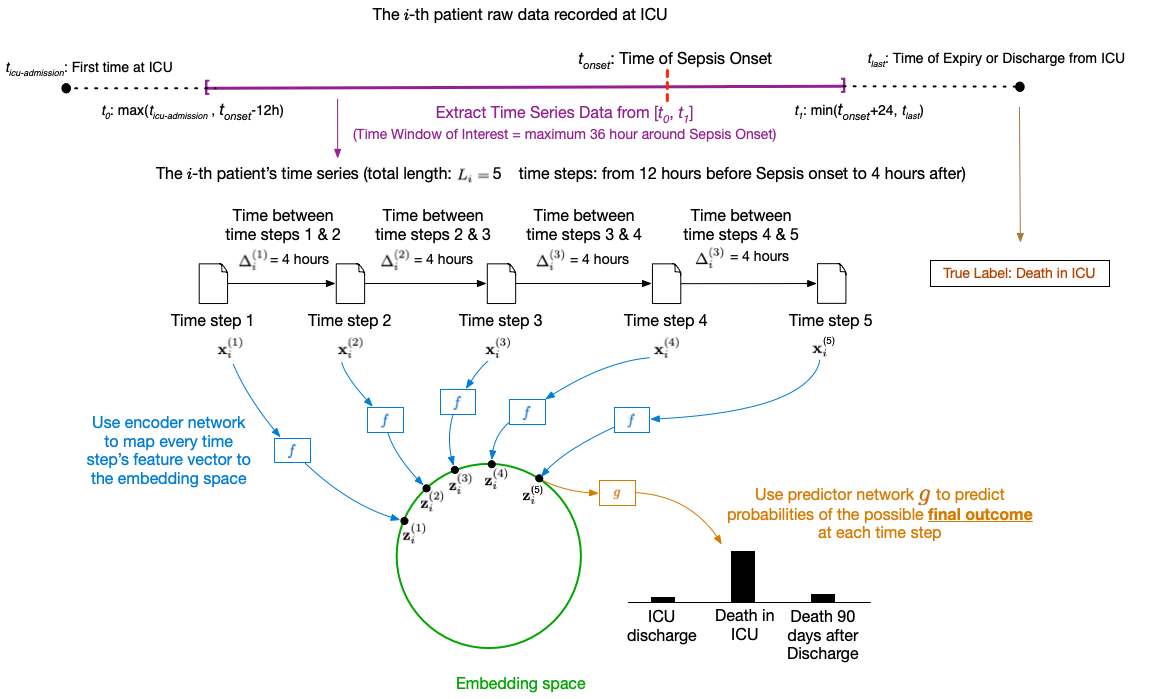
\includegraphics[width=.99\linewidth]{Appendices/appendix-ch02/images/MIMIC-Setup.png}
 \caption{Setup for MIMIC Experiments at Inference time from \ChTwoSmallCaps{Temporal-SCL}: First, we extract time series data for each patient from a time window around their sepsis onset within their complete ICU data timeline. This time series data is transformed into multiple time steps at 4-hour intervals. The resulting time series will have its features at each time step mapped onto the embedding space learned by our encoder. Finally, these resulting embeddings will be passed through our predictor network to predict the ICU mortality of each patient at every time step.
 }   \ChTwoFloatLabel{ch02:fig:mimic-setup}
\end{figure}



% !TeX root = ../../../main.tex
\begin{figure}[!ht]

\centering
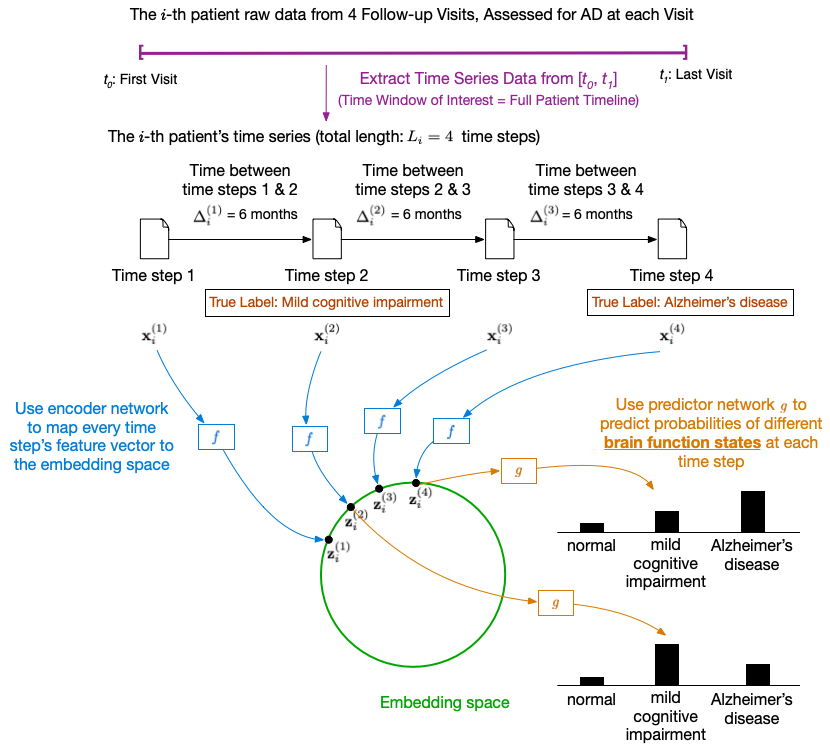
\includegraphics[width=.99\linewidth]{Appendices/appendix-ch02/images/ADNI-Setup.png}
 \caption{Setup for ADNI Experiment at Inference time from \ChTwoSmallCaps{Temporal-SCL}: First, we extract time series data for each patient from their complete timeline of available data spanning all the 6-month follow-up visits. This time series data maintains the same 6-month interval time steps as the raw data, with each time step having its own true class label representing one of the three possible brain function states. The resulting time series will have its features at each time step mapped onto the embedding space learned by our encoder. Subsequently, these resulting embeddings will be passed through our predictor network to predict the brain function class of each patient at every time step.
 }   \ChTwoFloatLabel{ch02:fig:adni-setup}
\end{figure}


\subsubsection{Real Data}
\label{ch02:sec:real-data-info}

\textbf{Medical Information Mart for Intensive Care (MIMIC).}
% \label{sec:data_mimic}
We consider the trajectory of septic patients using data from the Medical Information Mart
for Intensive Care (MIMIC-III) dataset (v1.4) \citep{johnson2018mimic}.
We follow the same procedure as done by \citet{komorowski2018artificial} to identify 18,354 septic patients among which there is an observed mortality rate just above 20\% (determined by death within 48h of the final observation $y_i^{(L_i)}=1$ or death within 90 days of the final observation $y_i^{(L_i)}=2$ versus discharge $y_i^{(L_i)}=0$).
From MIMIC, we extract demographic, lab results, and physiological features according to \citet{seymour2019derivation}, resulting in 29 features.
Note that Seymour et al.~group these features as follows: (1) Hepatic: Bilirubin, AST, ALT; (2) Hematologic: Hemoglobin, INR, Platelets; (3) Neurologic: GCS; (4) Cardiovascular: Heart rate, Systolic blood pressure, Bicarbonate, Troponin, Lactate; (5) Pulmonary: Respiratory rate, SaO2, PaO2; (6) Inflammatory: Temperature, ESR, WBC count, Bands, C-Reactive protein; (7) Renal: Serum creatinine; (8) Other: Age, Gender, Elixhauser, Albumin, Chloride, Sodium, Glucose, BUN. 
We compile the measurements recorded of these features in MIMIC for every 4 hours (duration of each timestep). 
Our temporal data extraction follows the exact experimental procedure as \citet{komorowski2018artificial} that is also adopted by \citet{killian2020empirical}.
Specifically, in the procedure that we followed, for the septic patients identified, we first found the time for the onset of sepsis based on Sepsis3 Criteria as $t_{\text{onset}}$, we then gathered recorded data of our selected features from the time 
$t_0 = \max(t_{\text{icu-admission}}, t_{\text{onset}}-12)$ to the time $t_1 = \min(t_{\text{icu-discharge}} \text{ or } t_{\text{death}}, t_{\text{onset}}+24)$.
This results in a maximum timeline $[t_0, t_1]$ of 36 hours worth of information captured from each patient (i.e. the maximum number of time steps would be 10 for a single patient) from $-12$ hours of the onset of sepsis to $+24$ hours afterwards.
We impute the missing values from the population median if a measurement is not recorded before and the previously recorded value if the measurement is recorded in a previous timestep. 
We also include a set of 26 indicators for our time-varying features at each timestep that tracks whether a measurement was recorded ($=1$) or imputed ($=0$).
This dataset represent the case where only the final outcome-label is known and non-terminal timesteps have unknown state-label.
Figure~\ref{ch02:fig:mimic-setup} shows the setup for our MIMIC-Sepsis experiment.


\noindent
\textbf{Alzheimer's Disease Neuroimaging Initiative (ADNI).}
% \label{sec:data_adni}
We also test our method on the Alzheimer's Disease Neuroimaging Initiative (ADNI) dataset \citep{petersen2010alzheimer}. 
This dataset consists of a total of 11,651 hospital visits from 1,346 patients which tracks the progression of Alzheimer's disease via follow-up observations at 6 months interval. 
Each patient has 21 variables out of which 5 are static and 16 are time-varying. 
The features include information on demographics, biomarkers of the brain function, and cognitive test results. 
These static features are as follows: (1) Demographic: Race, Ethnicity, Education, Marital Status; (2) Genetic: APOE$_4$.
The time-varying features include: (3) Demographic: Age, (4) Biomarker: Entorhinal, Fusiform, Hippocampus, Intracranial, Mid Temp, Ventricles, Whole Brain; and (5) Cognitive: ADAS-11, ADAS-13, Clinical Dimentia Rating Sum of Boxes (CDR-SB), Mini Mental State, Rey's Auditory Verbal Learning Test scores (RAVLT) Forgetting, RAVLT Immediate, RAVLT Learning, RAVLT Percent.
Following \citet{lee2020temporal}, we set our predictions on three diagnostic groups of normal brain functioning ($y_i^{(\ell)}=0$), mild cognitive impairment ($y_i^{(\ell)}=1$), and Alzheimer’s disease ($y_i^{(\ell)}=2$). 
The diagnostic is known at every timestep.
This dataset represent the case where we know the outcome-label at both terminal and non-terminal timesteps. 
Figure~\ref{ch02:fig:adni-setup} shows the overview for our ADNI experiment that follows \citet{lee2020temporal} setup.


\noindent
\textbf{Imputation.}
% \label{sec:imputation}
For both real datasets of this paper, we take the following approach to impute the missing features in our experiments. 
(1) For each patient, if at any time step feature has been recorded in a previous time step, we use the last recorded value to replace the missing feature.
(2) If at no previous time step a feature is recorded, we calculate the population median of the feature among all patients and impute the missing feature with this value.
In the future work, we aim to extend our approach to be similar to that of \citet{seymour2019derivation}, where multiple imputation with chained equations was used to account for missing data. 

In our MIMIC experiments, for each timestep, we include 26 indicators tracking measurement recording ($=1$) or imputation ($=0$) for time-varying features.


\subsubsection{Clustering on the Embedding Space for Our Visualization Strategy}
\label{ch02:sec:cluster}
For clustering on the embedding space, we use complete linkage Agglomerative Hierarchical Clustering. 
We first obtain the embedding representation of our training dataset and then train the clustering algorithm for $K\in\{5,7,8,9,10,14,20\}$. 
Subsequently, for predictive cluster assignment, we train a 3-Nearest Neighbor classifier (KNN) on the training data, utilizing the cluster assignments obtained in the previous step.
We use our classifier to get the predicted cluster assignment for the validation set. 


